% !TEX encoding = UTF-8 Unicode

\documentclass[twocolumn,10pt,a4j]{ltjsarticle}
\usepackage{kougai}

\title{Webサイトの最適な広告配置方法とテキストによる印象の調査}
\author{1932135 村上 航介  指導教員 須田 宇宙 准教授}
\date{}

\begin{document}

\maketitle

\section{はじめに}
%背景
近年,インターネット市場が年々需要が高まっているなか,広告において,TV・新聞などのマスメディアよりも,検索エンジン,Webサイト,アプリ,SNSなどインターネットを介して利用するメディアやサービスに広告を掲載する企業が増加している.また,インターネット広告自体のテキストのフォントの色使い,大きさなどの印象による宣伝効果への影響については明確になっていない.

%問題点
また,広告の配置によっては,ユーザにとって煩わしい位置にあるWebページが存在し,広告収益によるトレードオフを考えながら配置する必要がある.
これに対して,モバイル端末における広告配置についての研究があり,モバイル端末における有力な広告配置方法が挙げられている\cite{mobile}.
しかし,パソコン上での宣伝効果に適した広告配置が明らかになっていないという問題点があり,また,フォントによる印象についての研究は行われているが,広告におけるフォントに関する研究が行われていないことも問題となっている.

%目的
そこで本研究では,パソコン上に対して,Webサイトにおける広告配置とテキストによる煩わしさおよび宣伝効果の違いや影響を調査し,比較することを目的とする.

\section{インターネット広告}
2021年では,インターネット広告費がマスコミ四媒体広告費用(新聞/雑誌/ラジオ/テレビメディアの媒体費と製作費の合算)を上回ったことが報告されている\cite{dentsu}.

また,インターネット広告といっても様々な広告形態が存在し,そのなかでも,検索エンジンやWebサイト,アプリなどの広告枠に表示される画像,動画,テキスト広告のことを「ディスプレイ広告」という.
特徴としては,年齢や性別,過去のWebの閲覧履歴などをもとに,興味を持ってもらいたい層をターゲティングできる点が挙げられ,潜在層から顕在層に向けて幅広く訴求できる傾向にあるので,幅広い広告表現で視覚的に印象が与えられる.
%訴求:消費者の購買意欲に働きかける

\section{実験概要と結果}
本研究では,広告の配置とテキストのフォントによるパターンを分けて比較していくため,2回アンケートを行う.
配置のパターンとしては,画面右部・記事内・記事終わりで,それぞれのパターンで一つずつ記事に配置し,記事を見た後,アンケートに答えてもらう.
テキストのフォントでは,ゴシック体・明朝体・丸ゴシックで分けて,それぞれのパターンで一つずつ記事の広告として配置し,記事を見た後,アンケートに答えてもらう.
宣伝効果の指標として,表示されていた広告を正しく認識していたかどうかを回答する問題の正答率を用い,煩わしさの指標としては,4段階の評価の結果を用いる.
パソコンで見てもらうのを前提としているので,調査対象はパソコンを使用することが多い大学生を対象とする.

図\ref{fig:結果}では,配置とフォントによる煩わしさと宣伝効果(広告認識率)の調査結果で,横軸が宣伝効果,縦軸が煩わしさの大きさの割合を表しており,配置の煩わしさにおいては,記事内が最も高く,最も低いのは記事終わりという結果だった.
宣伝効果においては,記事終わりが最も高く,最も低いのは記事右部となった.

フォントの煩わしさにおいては,明朝体が最も多く,ほぼ同率でゴシック体と丸ゴシックが次に多かった.
宣伝効果においては,丸ゴシックが最も高く,最も低いのはゴシック体となった.

 
\begin{figure}[h]
\begin{center}
 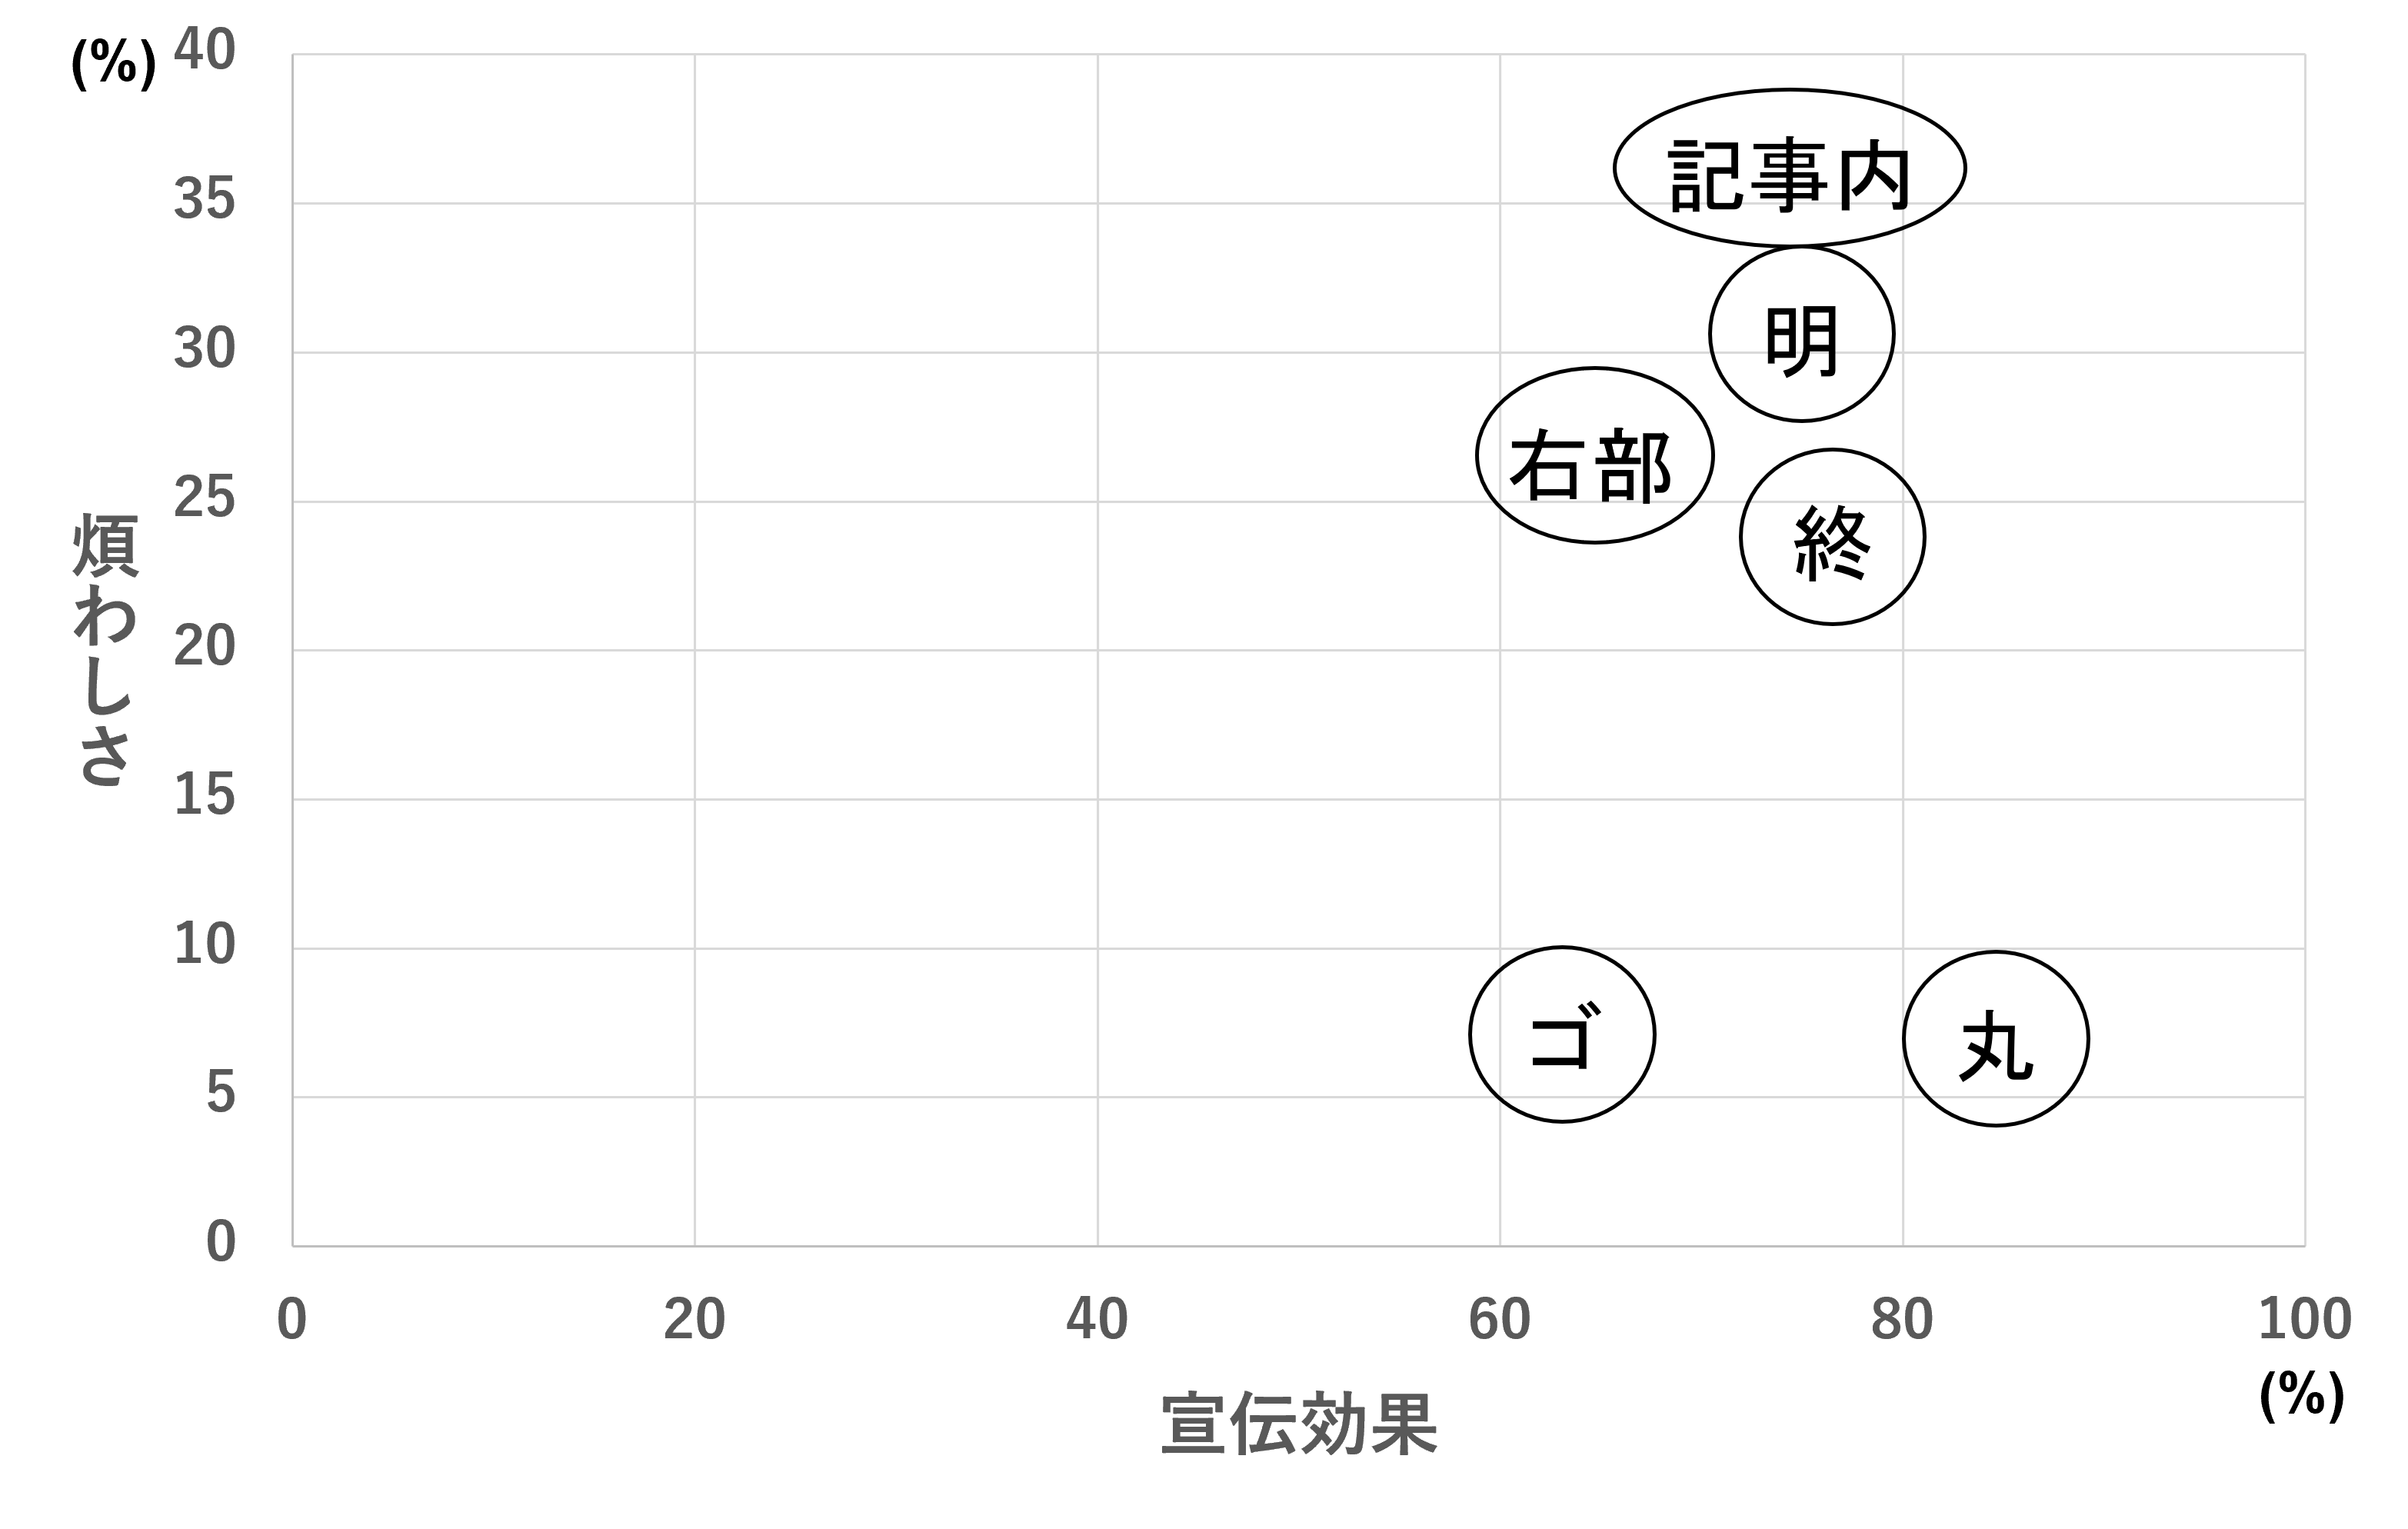
\includegraphics[height=50mm]{結果.png}
\end{center}
 \caption{配置とフォントのパターン分けの結果}
 \label{fig:結果}
\end{figure}

\section{考察とまとめ}
今回の結果から,煩わしさが高いため広告認識率も高いというわけではないことがわかり,パソコンにおける配置では,記事終わりが宣伝効果が高く,煩わしさが少ないことがわかった.
また,フォントにおいても丸ゴシックが最も煩わしさが少なく宣伝効果も高いことがわかり,パソコンにおけるインターネット広告の配置やフォントの違いによる煩わしさや宣伝効果の影響の違いを比較することができた.

\begin{thebibliography}{99}
\bibitem{mobile} 中島 弘貴,柗本 真佑,楠本 真二 ``モバイル端末におけるWeb広告の配置方法に対する一検討'',信学技報,vol.117,no.389,LOIS2017-62,pp.69-74,2018年1月
\bibitem{dentsu} 株式会社電通: ``2021年 日本の広告費'', \url{https://www.dentsu.co.jp/news/release/2022/0224-010496.html}, 2022/7/29参照
\end{thebibliography}

\end{document}